% Compile twice from docs/: pdflatex -interaction=nonstopmode -halt-on-error taximobile_pitch_deck.tex
% Technical briefing; normative requirements remain in the Markdown documents.
\documentclass[aspectratio=169,10pt]{beamer}
\usepackage[T1]{fontenc}
\usepackage[utf8]{inputenc}
\usepackage{lmodern,booktabs,tabularx,amsmath,tikz}
\usetikzlibrary{arrows.meta,positioning}
\definecolor{Navy}{HTML}{0B1F3A}
\definecolor{Mustard}{HTML}{D4A017}
\definecolor{Ink}{HTML}{283442}
\definecolor{Pale}{HTML}{F3F5F7}
\setbeamercolor{normal text}{fg=Ink,bg=white}
\setbeamercolor{structure}{fg=Navy}
\setbeamercolor{frametitle}{fg=Navy,bg=white}
\setbeamercolor{title}{fg=Navy}
\setbeamercolor{block title}{fg=Navy,bg=Mustard!25}
\setbeamercolor{block body}{fg=Ink,bg=Pale}
\setbeamertemplate{navigation symbols}{}
\setbeamertemplate{itemize item}{\color{Mustard}$\blacktriangleright$}
\setbeamertemplate{footline}{\hspace{5mm}\scriptsize TaxiMobile | Technical briefing | 6 September 2026\hfill\insertframenumber/\inserttotalframenumber\hspace{5mm}\vspace{3mm}}
\setbeamersize{text margin left=8mm,text margin right=8mm}
\newcommand{\src}[1]{\texttt{\scriptsize\detokenize{#1}}}
\newcommand{\refs}[1]{\vfill{\tiny\color{Navy}Repository: \detokenize{#1}}}
\title{TaxiMobile: architecture and delivery readiness}
\subtitle{Technical investment in a cooperative, city-governed taxi platform}
\author{Engineering assessment of the current working tree}
\date{6 September 2026}
\begin{document}
\begin{frame}
\titlepage
\begin{center}\textbf{84\% estimated engineering scope implemented}\par
Public launch / live pilot blocked; 0 of 19 P0 gates accepted\end{center}
\end{frame}

\begin{frame}{The engineering decision}
\begin{block}{Substantial implementation; incomplete operating evidence}
The repository contains shared passenger/driver apps, applicant and operations
web, authoritative ride/payment domains, city configuration and deployment tooling.
\end{block}
\begin{itemize}
\item 84\% is a weighted source-scope estimate, not test coverage or time spent.
\item Verified contacts, privacy self-service, payout accounting and governance controls still need work.
\item Hosting, providers, devices, security and staffed city acceptance remain open.
\item Next milestone: an immutable candidate and accepted staging, followed by bounded promotion.
\end{itemize}
\refs{docs/readiness.md; docs/gaps.md}
\end{frame}

\begin{frame}{What the audit includes}
\begin{columns}[T]
\begin{column}{.49\textwidth}
\textbf{Starting inventory}
\begin{itemize}
\item 922 project files, including untracked source.
\item 23 backend domain directories.
\item 48 Alembic migrations; head 0048.
\item 110 backend test files; 59 Kotlin test files.
\end{itemize}
\end{column}
\begin{column}{.49\textwidth}
\textbf{Evidence boundary}
\begin{itemize}
\item Structural and targeted critical-path review.
\item Fresh unit/API and source-contract checks.
\item Generated state and secrets excluded.
\item No hosted, legal, bank, real-device or remote-CI acceptance inspected.
\end{itemize}
\end{column}
\end{columns}
\begin{block}{Candidate identity}
Current dirty working tree over \src{f85417bcc8b432477fd88e87f5bd557a43898447};
that commit alone does not identify the tested implementation.
\end{block}
\end{frame}

\begin{frame}{Product constraints shape the architecture}
\begin{itemize}
\item Licensed taxi participation: an account is not a verified driver or city authorization.
\item Driver agency: deterministic dispatch and explicit acceptance; no invented surge incentives.
\item Supply privacy: no pre-assignment taxi markers, counts or candidate rankings.
\item Transparent economics: versioned tariffs, named fee base, explicit funding mode.
\item City rollout: independently configured and accepted operating jurisdictions.
\item Backend authority: identity, eligibility, assignment, pricing and payment status.
\end{itemize}
\begin{block}{Scope discipline}
Card/CMI, general chat, direct emergency dispatch and speculative scale services
must not be presented as launch capabilities.
\end{block}
\refs{docs/product.md; docs/operations.md; docs/payments.md}
\end{frame}

\begin{frame}{Four experiences, distinct authority}
\small
\begin{tabularx}{\textwidth}{@{}p{.18\textwidth}XX@{}}
\toprule Surface & Main workflow & Boundary \\\midrule
Passenger mobile & Estimate, request, track assigned ride, receipt, support & Own resources; no supply browsing. \\
Driver mobile & Apply, qualify, become available, accept, complete, earnings & Current account, vehicle, credential and city/service authority. \\
Applicant web & Recruiting city catalog, application, protected documents & Applicant-owned records; fail-closed upload dependencies. \\
Operations web & City configuration, review, money/cases, grants and audit & Active scoped staff permissions and operations MFA. \\
\bottomrule
\end{tabularx}
\refs{TaxiMobile/shared/; TaxiMobile/webApp/src/webMain/}
\end{frame}

\begin{frame}{Runtime topology}
\centering
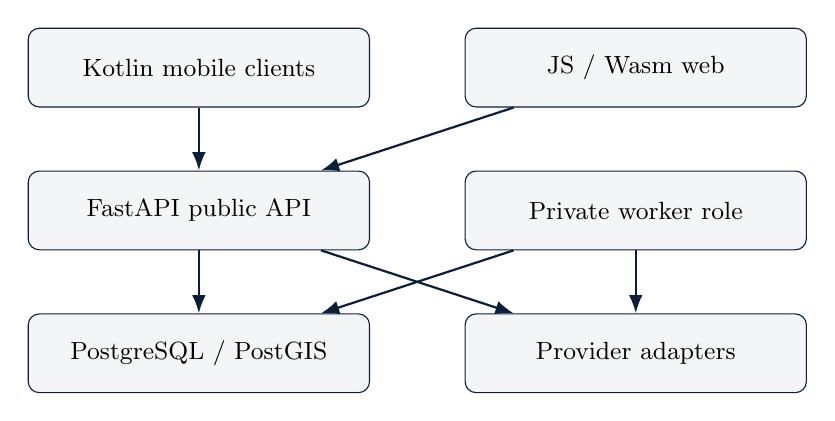
\begin{tikzpicture}[node distance=8mm and 12mm,
b/.style={draw=Navy,rounded corners,fill=Pale,align=center,text width=41mm,minimum height=10mm,font=\small},
a/.style={-{Latex},draw=Navy,thick}]
\node[b](m){Kotlin mobile clients};\node[b,right=of m](w){JS / Wasm web};
\node[b,below=of m](api){FastAPI public API};\node[b,right=of api](worker){Private worker role};
\node[b,below=of api](db){PostgreSQL / PostGIS};\node[b,right=of db](p){Provider adapters};
\draw[a](m)--(api);\draw[a](w)--(api);\draw[a](api)--(db);
\draw[a](worker)--(db);\draw[a](api)--(p);\draw[a](worker)--(p);
\end{tikzpicture}
\begin{block}{Source of truth}
Database transactions govern business state. Client caches and notification
payloads cannot acknowledge money or allocate a driver.
\end{block}
\end{frame}

\begin{frame}{Modular monolith and shared clients}
\begin{itemize}
\item Python FastAPI + SQLAlchemy/asyncpg + Alembic; PostGIS geographic authority.
\item API and worker are separate roles from the same backend image.
\item Transactional outbox and PostgreSQL fanout avoid premature queue/cache services.
\item Kotlin separates gateway/DTO, domain, coordinator, UI and native adapters.
\item Android passenger/driver flavors and iOS schemes share behavior without merging roles.
\item Browser applicant/operations roots are distinct from passenger/driver mobile composition.
\end{itemize}
\refs{docs/architecture.md; docs/implementation.md; backend/src/taximobile_api/}
\end{frame}

\begin{frame}{HTTP contract and unknown command outcomes}
\begin{itemize}
\item Stable \src{/api/v1} router; runtime OpenAPI describes mounted operations.
\item Fresh contract validation: 82 mobile HTTP + 1 WebSocket; 98 web HTTP operations.
\item The backend validates identity, scope, state, versions and required idempotency.
\item A timeout can occur after commit; it is not necessarily a rejected command.
\item Clients reload authoritative state and retain actionable errors; they do not automatically replay mutations.
\end{itemize}
\begin{block}{What route matching does not prove}
Payload compatibility, all authorization branches, full browser journeys and
provider/device delivery require additional tests.
\end{block}
\refs{infra/scripts/validate_mobile_api_contract.py; validate_web_api_contract.py}
\end{frame}

\begin{frame}{Identity and scoped staff security}
\begin{itemize}
\item Argon2 login, constrained JWT claims and current server-side session checks.
\item Revocation and suspension invalidate authority beyond token signature validity.
\item Operations uses separate sessions, scoped grants, MFA and recent-MFA boundaries.
\item Secure cookie/CSRF implementation exists; production acceptance remains separate.
\item Staff create/revoke UI now exists with typed confirmation and non-replay after MFA.
\end{itemize}
\begin{block}{Still incomplete}
Independent approval, authoritative staff lifecycle and last-admin continuity;
verified contact ownership and production recovery exercises.
\end{block}
\refs{domains/auth/; domains/administration/; GAP-005/020/022}
\end{frame}

\begin{frame}{Account recovery is explicit and bounded}
\begin{itemize}
\item Eight independent 100-bit offline codes after password reauthentication.
\item Domain-separated digests; 180-day expiry; one-time plaintext display for user custody.
\item Recovery consumes the complete set and revokes sessions/push in one transaction.
\item Staff cannot use the ordinary mobile recovery route.
\item Mobile saved-code acknowledgement, session listing/revocation and password change exist.
\end{itemize}
\begin{block}{Not yet delivered}
Verified email/phone ownership, delivery-based reset, self-service account deletion
and personal-data export. Offline codes do not establish verified contacts.
\end{block}
\refs{docs/auth.md; docs/security.md; GAP-020/021}
\end{frame}

\begin{frame}{Ride and offer state are different aggregates}
\small
\begin{block}{Successful live ride sequence}
REQUESTED $\rightarrow$ MATCHING $\rightarrow$ ACCEPTED $\rightarrow$
DRIVER\_EN\_ROUTE $\rightarrow$ DRIVER\_ARRIVED $\rightarrow$
IN\_PROGRESS $\rightarrow$ COMPLETED
\end{block}
\begin{itemize}
\item Offers separately track pending, accepted, declined, expired and cancelled states.
\item No ``OFFERED'' value is added to the implemented RideStatus enum.
\item Cancellation is restricted to documented pre-trip states; ordinary cancellation cannot erase an in-progress ride.
\item Completion finalizes fare and creates a pending payment; collection is separate.
\item Participant reads and coordination depend on backend-confirmed assignment.
\end{itemize}
\refs{domains/rides/models.py; domains/rides/service.py}
\end{frame}

\begin{frame}{Dispatch: discover, rank, lock, revalidate}
\begin{enumerate}
\item Discover a bounded geographic set satisfying account, vehicle, credential, city, service, availability and location conditions.
\item Rank deterministically using proximity, idle time and recent assignment signals.
\item Lock one candidate with skip-locked semantics rather than reserve all supply.
\item Recheck global account authority and eligibility after the lock.
\item Create the offer, or try another candidate / retry within the matching deadline.
\end{enumerate}
\begin{block}{Contention is not absence}
A temporarily locked candidate must not make the system falsely conclude that
the city has no eligible supply.
\end{block}
\refs{domains/matching/service.py; dispatch-contention integration cases}
\end{frame}

\begin{frame}{One active live ride per driver}
\[
\forall d:\quad |\{r:r.driver\_id=d\land r.status\in A\}|\leq 1
\]
\small
$A$ contains ACCEPTED, DRIVER\_EN\_ROUTE, DRIVER\_ARRIVED and IN\_PROGRESS.
\begin{itemize}
\item Migration 0048 creates a partial unique index on assigned drivers in active states.
\item It freezes ride writes and refuses existing conflicts instead of repairing history silently.
\item Service locks serialize supported commands; the index also rejects bypassing writes.
\item Immediate, scheduled and mixed-origin assignments must respect the same invariant.
\end{itemize}
\begin{block}{Acceptance gap}
Local race tests are not representative multi-replica city-load evidence.
\end{block}
\end{frame}

\begin{frame}{Published routes and scheduled bookings}
\begin{columns}[T]
\begin{column}{.49\textwidth}
\textbf{Fixed routes}
\begin{itemize}
\item Versioned direction, endpoints, stops, geometry and flat fare.
\item Publication is separate from driver supply.
\item Catalog visibility never promises a taxi.
\item Offers still require service authorization and acceptance.
\end{itemize}
\end{column}
\begin{column}{.49\textwidth}
\textbf{Scheduling}
\begin{itemize}
\item Reservation is separate from the live ride.
\item Policy defines horizon, opening, surcharge and cancellation.
\item Commitment/handoff recheck authority and location.
\item Rollback/replay must not duplicate live rides.
\end{itemize}
\end{column}
\end{columns}
\refs{domains/fixed_routes/; domains/scheduled_bookings/; scheduling integration tests}
\end{frame}

\begin{frame}{Exact and conserved financial components}
\small
Let $T$ be transport fare, $S=S_d+S_o$ scheduling surcharge and $F$ operator fee.
Let $a=1$ for passenger-funded fee, $a=0$ for driver deduction.
\begin{align*}
P &= T+S+aF & \text{passenger total}\\
D &= T+S_d-(1-a)F & \text{driver net}\\
O &= F+S_o & \text{operator allocation}\\
P &= D+O & \text{conservation}
\end{align*}
\begin{itemize}
\item Decimal arithmetic; half-up rounding to 0.01; defined transport-fare percentage base.
\item Currency, policy shape and driver-net floor validated server-side.
\item Policy versions and amounts snapshotted; later edits do not rewrite history.
\end{itemize}
\refs{domains/pricing/service.py::calculate_financial_quote}
\end{frame}

\begin{frame}{Money example: funding mode changes the receipt}
\begin{block}{Illustrative arithmetic, not an approved tariff}
$T=100.00$, scheduling surcharge $S=0$, operator fee $F=10.00$.
\end{block}
\begin{center}\begin{tabular}{lrrr}
\toprule Funding mode & Passenger & Driver net & Operator \\\midrule
Driver deduction & 100.00 & 90.00 & 10.00 \\
Passenger surcharge & 110.00 & 100.00 & 10.00 \\\bottomrule
\end{tabular}\end{center}
\begin{itemize}
\item Both conserve passenger total into driver and operator allocations.
\item Client estimates must not invent a fee base or hide the deduction.
\item An earning allocation is not proof of a payout or a bank transfer.
\end{itemize}
\refs{docs/pricing.md; docs/payments.md}
\end{frame}

\begin{frame}{Payment settlement requires a separate authority}
\begin{itemize}
\item Ride completion creates one pending payment.
\item Cash: authorized driver confirms collection; receipt initially remains pending.
\item Manual transfer: passenger claims; scoped staff reconciles exact external evidence.
\item Processing means awaiting review, never ``paid''.
\item Non-legacy cities resolve active versioned capabilities and recipient instructions from the exact city bundle.
\item Card/CMI is deferred; reserved enum values are not advertised payment options.
\end{itemize}
\refs{domains/payments/; versioned-payment and cash-workload tests}
\end{frame}

\begin{frame}{Refunds exist; payout accounting does not}
\begin{columns}[T]
\begin{column}{.49\textwidth}
\textbf{Implemented refunds}
\begin{itemize}
\item Append-only, completed-payment linkage.
\item Exact positive amount and bounded cumulative total.
\item Locking, idempotency, reason, evidence and audit.
\item Full operator funding; zero driver recovery.
\end{itemize}
\end{column}
\begin{column}{.49\textwidth}
\textbf{GAP-024}
\begin{itemize}
\item Settlement periods and payable balance.
\item Cash offsets and payout instructions.
\item Remittance/reconciliation ledger.
\item Accountant-approved correction and dispute policy.
\end{itemize}
\end{column}
\end{columns}
\begin{block}{Decision dependency}
Approve accounting policy before introducing payout schema or silently reusing earnings as a ledger.
\end{block}
\end{frame}

\begin{frame}{Durable effects and refresh-only notifications}
\begin{itemize}
\item Transactional outbox keeps delivery work associated with committed business state.
\item PostgreSQL fanout serves multiple connected API instances.
\item WebSocket and FCM/APNs hints trigger authorized reads.
\item Invalid registrations, bounded retries, dead letters and reviewed replay are explicit paths.
\item Payloads and logs must avoid exact location, transfer instructions and safety narratives.
\end{itemize}
\begin{block}{Failure interpretation}
No notification does not mean no commit. A delivered notification is not
independent authority for assignment or settlement.
\end{block}
\refs{domains/outbox/; core/live_events.py; integrations/push/}
\end{frame}

\begin{frame}{Eight background loops need observable progress}
\small
\begin{tabularx}{\textwidth}{@{}lX@{}}
\toprule Loop & Operational responsibility \\\midrule
Matching & Dispatch progression and expiry/retry. \\
Outbox & Durable delivery and failure recovery. \\
Credentials & Eligibility lifecycle. \\
Scheduling & Due reservations and live handoff. \\
Analytics & Aggregate projection refresh. \\
Case alerts & Overdue support/safety escalation. \\
Case retention & Eligible minimization with hold protection. \\
Document retention & Protected-file lifecycle through configured storage. \\
\bottomrule
\end{tabularx}
\vspace{2mm}Readiness requires supervisor health and positive loop progress; liveness alone is insufficient.
\refs{workers/application.py; production readiness and monitoring validators}
\end{frame}

\begin{frame}{Maps and locations: source versus service quality}
\begin{itemize}
\item MapLibre native composition, neutral fallback and shared route/point overlays.
\item Valhalla/GraphHopper adapters behind a selected backend routing contract.
\item Authenticated normalized place search/reverse lookup with PostGIS pickup authority.
\item One-shot location plus foreground-only online driver heartbeat are implemented.
\item Continuous background tracking is not implied by that heartbeat.
\end{itemize}
\begin{block}{Open acceptance}
Real graph/style/geocoder, data/license and query privacy, multilingual search,
device battery/network behavior and accepted Arabic routing narration.
\end{block}
\refs{GAP-006/007/008/026; native location and MapLibre source sets}
\end{frame}

\begin{frame}{Mobile and browser quality are separate test boundaries}
\begin{itemize}
\item Shared coordinators improve consistency; native lifecycle and permissions still differ.
\item English/French/Arabic catalog parity does not prove accessibility or RTL layout.
\item Backend-confirmed success drives UI feedback; unknown outcomes retain recovery paths.
\item JS/Wasm component tests do not establish complete hosted applicant/staff journeys.
\item Windows JVM verification cannot execute iOS simulator tests.
\item Signed release, provider config, R8/dSYM and controlled crash evidence remain gates.
\end{itemize}
\refs{docs/design.md; docs/ui.md; docs/extended_ui.md; GAP-013/014/025}
\end{frame}

\begin{frame}{City configuration is a coherent versioned bundle}
\begin{itemize}
\item Market $\rightarrow$ city/operator assignment $\rightarrow$ enabled service.
\item Service area, tariff, fee, scheduling and payment references must be compatible.
\item Fixed-route publication and driver authorization stay service/city scoped.
\item Operations UI resolves backend versions rather than constructing authority in the browser.
\item Readiness, pause/resume and closeout controls exist in source.
\end{itemize}
\begin{block}{Governance limit}
Valid evidence records do not prove that the uploaded legal evidence is true,
the recruited cohort is eligible or the duty roster will answer.
\end{block}
\refs{docs/operations.md; domains/markets/; operations web control plane}
\end{frame}

\begin{frame}{Documents, support and safety need real operators}
\begin{itemize}
\item Protected application PDF/JPEG/PNG workflow fails closed without storage/scanning.
\item Scoped reviewer access, encrypted document boundary and retention code exist.
\item Support and restricted safety records have separate visibility and triage.
\item Overdue paging, acknowledgement, legal holds and minimization are implemented.
\item Platform safety reporting does not place emergency calls or dispatch help.
\end{itemize}
\begin{block}{Acceptance includes people and every store}
Real scanner/key operation, trained shifts, pager drills, incident response and
backup/log/provider expiry must be demonstrated.
\end{block}
\refs{GAP-011/012/017/030/031}
\end{frame}

\begin{frame}{Production manifests are not deployed infrastructure}
\begin{itemize}
\item Separate API/worker roles, restricted operations ports and readiness boundaries.
\item Bounded JSON logs and authenticated aggregate metrics.
\item Prometheus, Alertmanager, Loki, Alloy and Grafana overlay/validators.
\item Migration/backup/restore and deployment-verification scripts.
\item CI provenance, contract checks and image supply-chain definitions.
\end{itemize}
\begin{block}{Not established by source files}
Accepted host/region, TLS/DNS, private networks, secret rotation, immutable registry,
managed recovery, real monitoring targets, pager ownership or HA.
\end{block}
\refs{infra/deploy/; infra/scripts/; .github/workflows/ci.yml}
\end{frame}

\begin{frame}{Restore and migration must match the candidate}
\begin{itemize}
\item Current schema head: \src{20260903_0048}, 48 ordered migrations.
\item Offline SQL generation is not a live lock/permissions/historical-data rehearsal.
\item Older documented restore at 0029 remains historical, not a current-head result.
\item Required: isolated 0048 restore, integrity/readiness checks and measured recovery.
\item RPO/RTO, retention, encryption and legal-hold implications need approved ownership.
\item Forward-fix/rollback must respect schema compatibility and irreversible data changes.
\end{itemize}
\refs{GAP-003; docs/database.md; infra recovery scripts}
\end{frame}

\begin{frame}{Fresh checks and historical evidence}
\small
\begin{tabularx}{\textwidth}{@{}p{.38\textwidth}X@{}}
\toprule Check & Result / qualification \\\midrule
Backend unit/API & 699 passed; 173 deprecation warnings; 45.52 seconds. \\
Infrastructure/mobile script tests & 11 + 30 passed. \\
Mobile/backend contract & 82 HTTP + one WebSocket passed. \\
Web/backend contract & 98 HTTP operations passed. \\
Shared JVM forced rerun & 178 passed; zero failures/errors/skips. \\
Full fresh-PostGIS suite & Existing record: 819 passed; not rerun for this documentation assessment. \\
Native/hosted/remote CI acceptance & No fresh acceptance claimed. \\
\bottomrule
\end{tabularx}
\refs{docs/readiness.md for commands, scope and final verification}
\end{frame}

\begin{frame}{How the 84 percent estimate is calculated}
\begin{block}{Explicit source-scope rubric}
0 requirement only; 1 scaffold; 2 material implementation with a major missing
workflow; 3 main path/tests with meaningful remaining scope; 4 defined core
source path and meaningful boundary tests.
\end{block}
\[
 C=\sum_i w_i(s_i/4)=336/4=84\%,\qquad \sum_i w_i=100.
\]
\begin{itemize}
\item Weights are assessment judgments, not approved budgets or elapsed effort.
\item Approximately 75--90\% sensitivity range; not a statistical confidence interval.
\item Deferred products excluded; identified launch engineering gaps included.
\item P0 acceptance is a veto, not another weighted score: 0/19 accepted.
\end{itemize}
\end{frame}

\begin{frame}{Implementation matrix: core domains}
\small
\begin{tabularx}{\textwidth}{@{}Xrrr@{}}
\toprule Workstream & Weight & Rating / 4 & Contribution \\\midrule
Identity/recovery & 8 & 3 & 6.00 \\
Drivers/recruitment & 8 & 4 & 8.00 \\
Immediate rides/coordination & 10 & 4 & 10.00 \\
Matching/integrity & 8 & 4 & 8.00 \\
Pricing/economics & 7 & 4 & 7.00 \\
Payments/settlement & 8 & 3 & 6.00 \\
Fixed routes/scheduling & 7 & 4 & 7.00 \\
\bottomrule
\end{tabularx}
\vspace{3mm}Missing verified contact and payout paths cap their workstreams below four.
Four indicates source/tests, never field or financial acceptance.
\refs{docs/readiness.md: evidence and missing scope per row}
\end{frame}

\begin{frame}{Implementation matrix: clients and enabling systems}
\small
\begin{tabularx}{\textwidth}{@{}Xrrr@{}}
\toprule Workstream & Weight & Rating / 4 & Contribution \\\midrule
Mobile & 10 & 3 & 7.50 \\
Web & 7 & 3 & 5.25 \\
Maps/places/navigation/delivery & 6 & 3 & 4.50 \\
Support/safety & 5 & 3 & 3.75 \\
Control plane/governance & 5 & 3 & 3.75 \\
Privacy rights/lifecycle & 4 & 2 & 2.00 \\
Analytics & 2 & 3 & 1.50 \\
Deployment/observability & 3 & 3 & 2.25 \\
CI/supply chain/release & 2 & 3 & 1.50 \\\bottomrule
\end{tabularx}
\refs{Combined weights = 100; combined contribution = 84.00}
\end{frame}

\begin{frame}{Engineering gaps to resolve before claiming completion}
\begin{enumerate}
\item Verified contacts and production recovery: choose/approve identity and delivery behavior.
\item Privacy self-service: deletion/export with legal holds and cross-store consequences.
\item Staff governance: independent approval and last-admin continuity.
\item Settlement accounting: periods, balances, cash offsets, remittance and reconciliation.
\item Complete client/provider integration: narration, device/browser journeys and failure behavior.
\end{enumerate}
\begin{block}{Policy before schema}
The audit records these dependencies; it does not invent accounting, legal,
recovery or major authorization rules to accelerate a percentage.
\end{block}
\refs{GAP-020--024; GAP-025/026/030}
\end{frame}

\begin{frame}{Evidence-based delivery sequence}
\begin{enumerate}
\item Review uncommitted work; identify a clean candidate and immutable artifacts.
\item Resolve policy-dependent software scope in owning domain documents.
\item Accept isolated staging, current-head restore and selected providers.
\item Complete device/browser, independent security and defined capacity gates.
\item Train scoped operators and rehearse money, safety, paging and recovery.
\item Promote to bounded field validation, pilot and public city only with explicit acceptance.
\end{enumerate}
\refs{docs/workflow.md; docs/testing.md T0--T10; docs/gaps.md}
\end{frame}

\begin{frame}{A task is one complete behavior slice}
\begin{itemize}
\item Start: requirement/GAP, actor/scope, trigger, outcome and rejected cases.
\item Trace existing architecture and implementation before adding code.
\item Define transaction, schema/API impact and meaningful negative/failure tests.
\item Connect shared gateway/coordinator and native adapter with honest UI state.
\item Update owning docs; run checks at the changed boundary.
\item Handoff: source/artifact identity, commands, observed results, limits and open gates.
\end{itemize}
\begin{block}{Conflict rule}
Pause the affected implementation if normative requirements conflict with code;
do not rewrite policy to approve a convenient implementation.
\end{block}
\end{frame}

\begin{frame}{Promotion needs traceable evidence}
\small
\begin{tabularx}{\textwidth}{@{}lX@{}}
\toprule Stage & Necessary evidence boundary \\\midrule
T0--T2 & Source/static, unit/component and simulated-persona contracts. \\
T3 & Isolated migrated PostGIS and multi-role system transactions. \\
T4 & Browser, emulator and physical-device lab. \\
T5 & Candidate staging: restore, providers, security and realistic load/failure. \\
T6 & Trained staff, synthetic cases, money and incident rehearsal. \\
T7--T8 & Approved bounded field validation then real-user pilot. \\
T9--T10 & Public city acceptance, closeout and proven repeatable expansion. \\
\bottomrule
\end{tabularx}
\vspace{3mm}Record owner, date, candidate/artifacts, schema, city/provider versions,
scenario, observed result, evidence location, expiry and decision.
\end{frame}

\begin{frame}{Documentation now has a clearer division of responsibility}
\begin{itemize}
\item \src{readiness.md}: dated percentage, matrix, findings and fresh/historical results.
\item \src{workflow.md}: task contracts, commands, handoffs and promotion sequence.
\item \src{gaps.md}: detailed open-work closure and acceptance criteria.
\item \src{testing.md}: T0--T10 scenarios; workload companion for guarded HTTP experiments.
\item Domain docs retain product, API, schema, security and UI authority.
\item TeX/PDF reports communicate the assessment and must track the same evidence date.
\end{itemize}
\refs{docs/README.md is the entry point}
\end{frame}

\begin{frame}{Decision requested from the project owner}
\begin{block}{Prioritize an accepted operating system around the source}
The next work is candidate consolidation, policy-dependent completion and staged
acceptance for one bounded city, with explicit owners and measurable stop criteria.
\end{block}
\begin{itemize}
\item Keep the implemented modular architecture and backend authority boundaries.
\item Resolve settlement/privacy/identity/governance decisions before coding those gaps.
\item Identify infrastructure, security, provider, city, payment and safety owners.
\item Require evidence at each promotion gate; do not equate 84\% source scope with permission to launch.
\end{itemize}
\refs{Communication artifact only; no deployment or policy approval is implied.}
\end{frame}
\end{document}
